%!TEX root = ../crimson_throne_book_main.tex
% 2016-06-11
Vencarlo talks to the distraught Leroung family and convinces them to join the heroes to the rebel base. They place Lady Eliasia's body on a hand drawn cart and make their way to the graveyard in the Gray District as a funeral procession. Puk scouts ahead and Vencarlo follows behind; both of them are on the look-out for possible sources of trouble, ready to interfere when necessary. Still, since the streets are a lot more crowded today than they have been in weeks, it is rather easy to get south undisturbed. The Leroung family take their dead mother to bishop Keppira d'Bear, to make arrangements for her burial. In the meantime Vencarlo leads the party to the rebel hideout, underneath a crypt in the graveyard. He tells them the church of Pharasma is in on the conspiracy, supporting the rebels as best they can without compromising their own safety.\\

\hyperref[fig:Rebel-base-in-Korvosa-Curse-of-the-Crimson-Throne-614606623]{ The hideout is cramped with people who have fled prosecution, a fair number of young girls who were drafted for the Gray Maiden forces among them. } Vencarlo introduces the party members to Illrem Bromathan, the leader of the resistance, a former Sable Company officer. Illrem is brother to Lord Valdur IV, who has been arrested for being allied to House Endrin and being a staunch supporter of the Sable Company. No one has heard of him since his arrest, and Illrem can only hope that Valdur's position as a priest of Sarenrae has kept him alive so far. Valdur's wife and son have been placed under house arrest and are still residing in the family home under Gray Maiden guard, much like the Leroung family was. Illrem's second-in-command is a young man whom the companions already know: Aaron Endrin, the son of the former commander of the Sable Company, Marcus Endrin, who was killed at the hands of the Queen herself. Sjo tells the rebels about the blood clone Maidens, which gets Illrem quite worried. The girls who have been recruited have all been brought to the temple of Asmodeus. Quint remembers from their earlier meeting with Archbishop Ornher Reebs of Asmodeus that the high priest seemed to know more about the cloning process, when they took Dame Nesia to the temple. The party and their rebel friends now fear that the recruits are being sacrificed in the temple to create the blood clone army. If this is the case, they will have to put an end to this vile practice as soon as possible. \\

\begin{figure}[h]
	\centering
	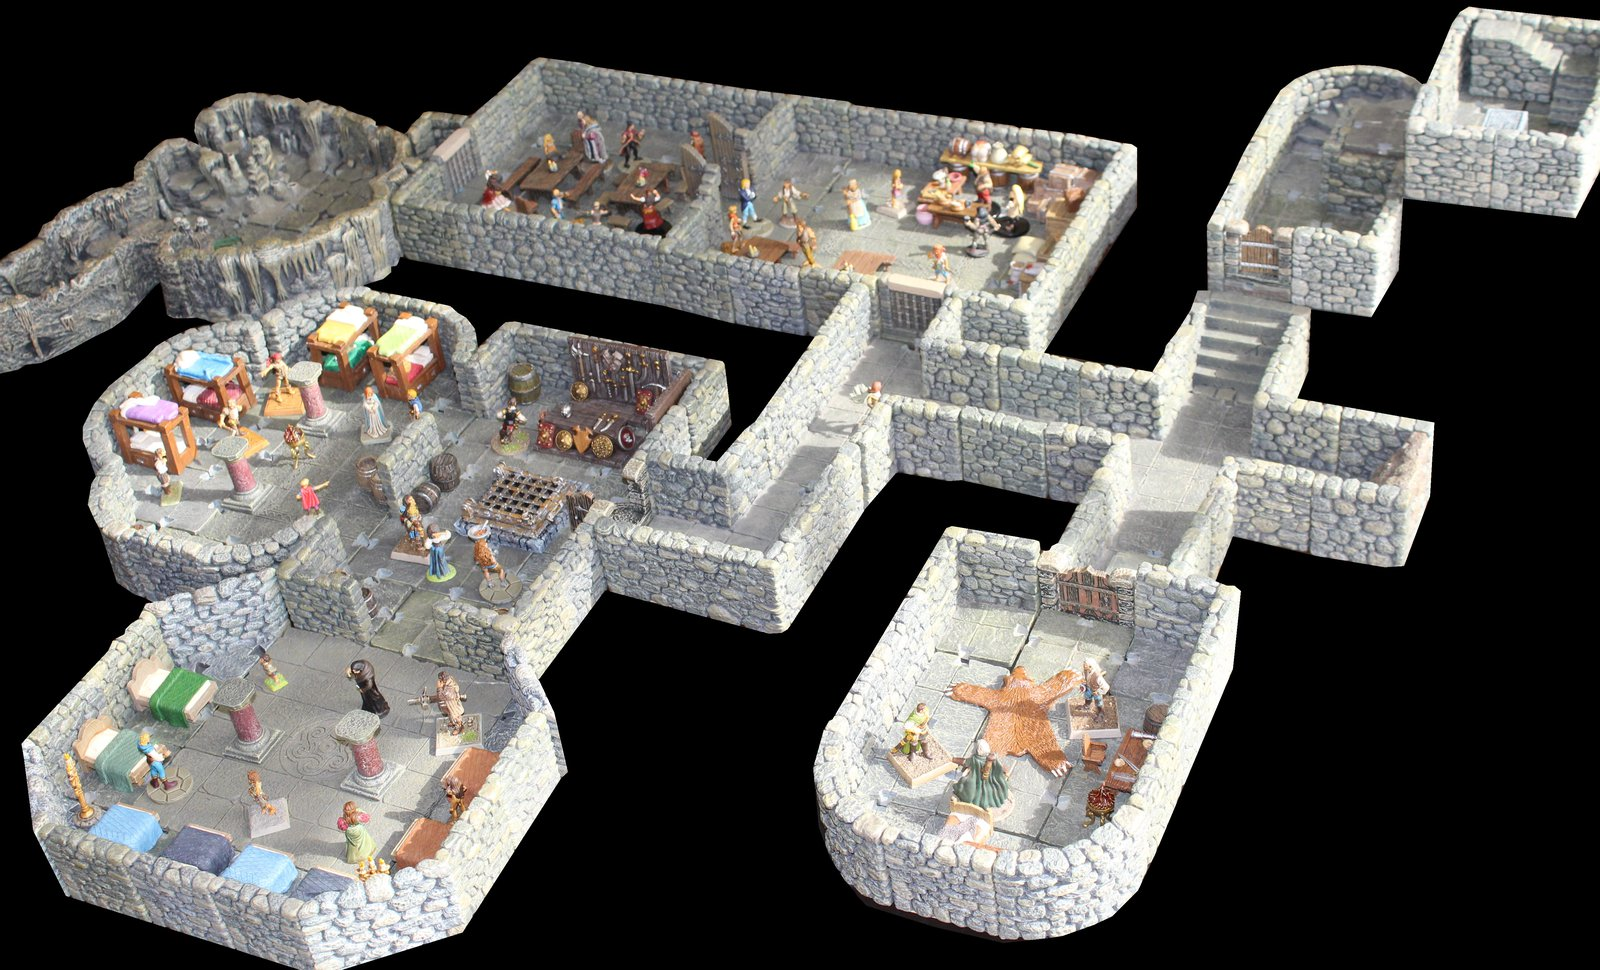
\includegraphics[width=0.39\textwidth]{images/Rebel-base-in-Korvosa-Curse-of-the-Crimson-Throne-614606623.jpg}
	\caption{Rebel base in Korvosa Curse of the Crimson Throne}
	\label{fig:Rebel-base-in-Korvosa-Curse-of-the-Crimson-Throne-614606623}
\end{figure}

Balian questions this approach, though. He wonders if it is worth it exposing themselves, when most recruits are probably dead already. This practice must have been going on for weeks already. How many girls can be left to save? Quint argues that getting revenge for such an enormous evil in itself is worth it, even if there is no one left to save. Balian agrees, but asks for 'carte blanche' when they invade the temple to kill anyone he wants. He fears that capturing someone like Reebs is dangerous, only killing him will prevent him from escaping. Although Quint feels it is very likely that Reebs will lose his life in the raid, he finds it wise to try and question enemies first. If Reebs is one of Ileosa's most powerful allies, he could be a valuable source of information. 'Kill first, ask questions later' does not work, so the bard suggests to ask the questions first. Killing the man afterwards is a very viable option!\\

Suddenly Sjo looks like he's slipping into a mini-trance. He hears Thousand Bones' voice in his head. The Shoanti shaman tells him preparations in the Cinderlands are still on schedule and asks if they should proceed according to the agreed-upon timing. Sjo answers that there is no trace of the ancient shaman's grave yet and that things are chaotic, but the timing is still okay.\\

After Thousand Bones' {\itshape sending} , the companions decide to stake out the temple of Asmodeus. They head to the other side of the city during the evening hours. There are six Gray Maidens in front of the temple doors. Their military stance and synchronous movements suggest they are blood clones. In the next half hour, no one enters the temple, but seven Gray Maidens come out and head into the city. Quint wants to try and get inside, preferably under cover. The Old Courthouse, where the companions spent one night of horror a couple of months ago, is the only safe place nearby he can think of to change into a disguise. Quint finds an old barrister's robe in the building, cleans it up with  {\itshape prestidigitation} and puts it on over his clothes. He also puts on make-up to change his appearance. Now he looks like a lawyer, a perfect disguise to gain entry to the temple of the god of contracts. Quint approaches the Gray Maidens at the gate and convinces them to let him through. \hyperref[fig:Temple-of-Asmodeus-in-Korvosa-614608557]{ The temple itself looks empty inside. } Quint sits down on one of the pews and starts praying. A few minutes later a woman exits from the side chapel and walks up to the late guest. She questions him about his identity. The bard claims to be a lawyer who has recently arrived from Cheliax. He is looking for clients and wouldn't mind defending people who are not goody two-shoes \ldots after all, everybody has the right to a good defense. You'd be amazed at what the law allows, even in bureaucratic places like Cheliax and Korvosa. The priestess smiles, but she strongly recommends that he read up on the many Korvosan laws and charters, for they are 'many' indeed! When Quint asks about the guards at the door, the priestess explains that things in the city have been quite hectic of late. The church of Asmodeus has openly joined the queen's side and is possibly in danger from the queen's enemies now, so they have been granted a number of royal guards. \\

\begin{figure}[h]
	\centering
	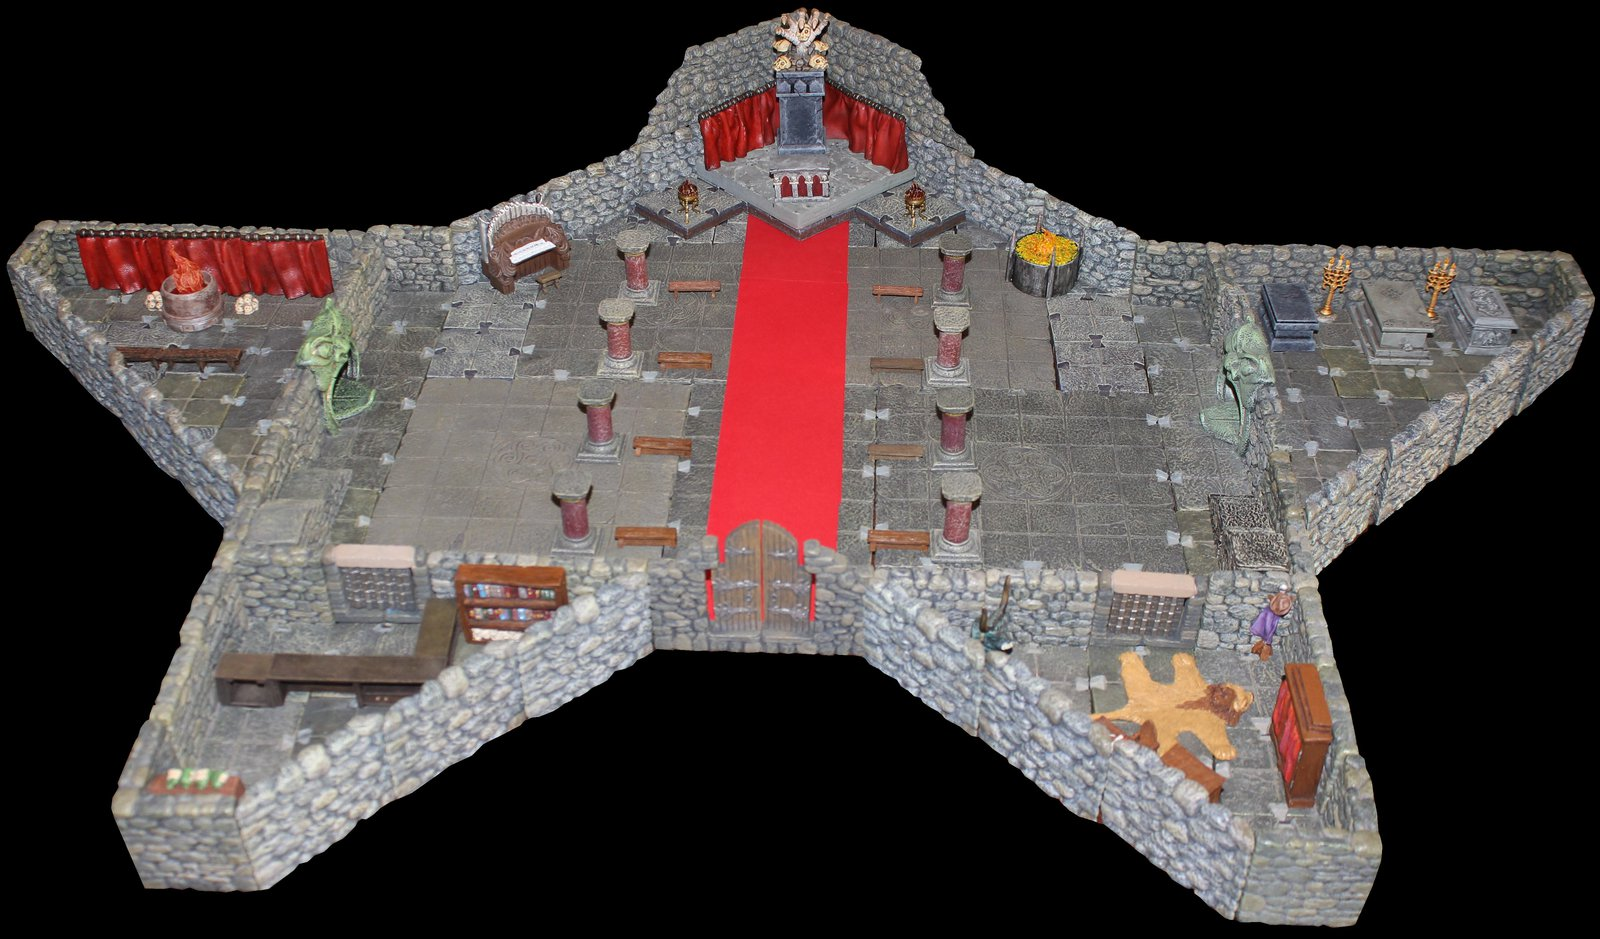
\includegraphics[width=0.39\textwidth]{images/Temple-of-Asmodeus-in-Korvosa-614608557.jpg}
	\caption{Temple of Asmodeus in Korvosa}
	\label{fig:Temple-of-Asmodeus-in-Korvosa-614608557}
\end{figure}

When Quint enquires about the church's leader, Ornher Reebs, he notices some malcontent in the woman's eyes. She tell him the archbishop is not available at the moment. Quint presses the matter and tries to find out more about the high priest, especially from the priestess's perspective. The woman, whose name is Tyresha, does admit that she might see herself following in Reeb's footsteps one day, but for now the man has things tightly under control in the temple. Quint suggests that there are other ways to help fate along, but Tyresha shies away from the idea of killing her leader. {\itshape``It is not killing I refer to,}'' Quint quickly clarifies, {\itshape``but using the law.}'' He links back to one of Reebs' earliest deeds here in the city: the sacrifice of thirteen virgins. True, Asmodeus does consent with the occasional sacrifice, but he also has the sense to follow the laws of the land first. Such a sacrifice is indeed possible in Cheliax, but not in Korvosa. The city's reaction to his imprudent offer almost got Asmodeus kicked out when he had just managed to get his foot in the door. If it hadn't been for Queen Domina's interference and the resurrection of most of the girls at her expense, Asmodeus would have been ousted from here before his temple was completed.\\

{\itshape``I just hope Reebs isn't repeating the same stupidity before Korvosa --and especially its laws -- are ready for it}'', Quint goes on. Again he detects a hint of doubt in the priestess's eyes. {\itshape``In the eyes of the father church, such deeds would be considered 'wrong', not necessarily for being against church policy as such, but for discrediting the name of Asmodeus in a place where his worship is -- let's be honest -- barely allowed. If this leads to the church being abolished from these lands, Asmodeus loses. And our Lord does not like to lose. Those responsible would have to be brought to church justice, which is actually the real reason why I am here.}''\\

{\itshape``You are an inquisitor, then?}'' Tyresha gasps.\\

{\itshape``Indeed, I am}'', Quint bluffs, seeing that the priestess totally buys his bluff.\\

{\itshape``Well, suppose I could give you information about the archbishop, could you make sure it serves my purposes as well?}'' she asks.\\

{\itshape``I do not have the power to name a new archbishop, but I would make sure that the father church knows about your loyalty. As you know, the Prince of contracts is a big fan of loyalty, I have no doubt it \ldots you would be rewarded}'', Quint tells her. {\itshape``If the wrong-doings of the past were to repeat themselves, it would not bode well for Reebs, I can assure you.}''\\

{\itshape``I suggest we move to the chapel}'', Tyresha whispers. {\itshape``It has been protected from eaves-dropping, if we want to negotiate contracts with potential 'clients', you see. It will be safer to talk there.}''\\

The priestess leads Quint to the side chapel to continue the conversation: {\itshape``So, to make sure I understand you correctly, if I could confirm ill tidings about Reebs, you could help me rise to power in Korosa's temple?}''\\

{\itshape``I will definitely use all my influence in the church to see that happen}'', Quint confirms.\\

Tyresha smiles. {\itshape``Well then, there is much I can tell you. The archbishop has been executing very extreme rituals in the basement, even for Asmodean standards. He's been sacrificing numerous young girls, bleeding them completely dry to use their life's blood to create an army of clones. He infuses these creatures further with devil blood and uses a special construct, called an 'akaruzug', to draw upon the talents of an accomplished 'original' and turn his creations into very skillful fighters.\\

He has four Erinyes and one hamatula - or barbed devil - aiding him in this process. These servants have not been provided by Reebs himself, though, but rather by the queen, who has secured the servitude of a fair number of devils through an infernal contract. Judging by the number and strength of these devils alone, this contract must be one of the most powerful ones I have ever heard about. And her majesty did not sign it here, either, but at the Acadamae. Our school of wizards is known for its intimate dealings with devils, as I'm sure you know.}''\\

{\itshape``You wouldn't happen to have seen a copy of said contract?}'' Quint wonders.\\

{\itshape``The queen would be stupid to show this precious document to anyone. She probably keeps her copy hidden away in the castle, in a place no one can get to. The other copy is, obviously, still in the hands of the contract devil who made the agreement. I can't even guess who he is, though someone in the Acadamae must know.}''\\

{\itshape``Naturally}'', Quint nods.\\

{\itshape``We all know Asmodeus works in mysterious ways. His contract dealers might indeed sign papers that allow an individual to control devils and command them to act in whichever way he or she desires, even if this would not be Asmodeus's chosen path. On the other hand, in such cases Asmodeus would support efforts to see the contract fail its owner. After all, isn't that why he likes to include loopholes in his contracts? Fooling mortals into thinking they gain great power, only to have the contract bite them in the ass and reap their souls prematurely?}''\\

{\itshape``You understand our Lord's teachings well. You would make a great successor for Reebs, indeed}'', Quint acknowledges. {\itshape``You will understand that I did not come to this city alone. I have a number of bodyguards waiting outside. I'm afraid I will have to return to bring Reebs's wrong-doing to justice. Is there any way you can facilitate our entry?}''\\

{\itshape``Of course there is, master inquisitor. I will leave the front doors unlocked and I will tell the guards at the door to let you through. You will find Ornher Reebs in the basement. I suspect he will be there all night}''\\

{\itshape``Excellent, you should make sure you are nowhere about when we come in. It would be best if your role in this mess remains unnoticed. It is enough that I know of your loyalty so I can relay it to our leaders in Cheliax when the time is right}'', Quint finishes.\\

Confident she has struck a great deal, Tyresha shows the disguised bard out and informs the guards at the door that they should let the inquisitor in whenever he wants. After that Quint disappears into the night and reunites with his friends afew moments later. He feels quite happy to prove Balian wrong: words often are more powerful than the blade! Now at least the companions can prepare for the challenges ahead.\\

